% IEEE OJVT template (ieee-ojvt.cls, 2024-06-27, from the IEEE Template Selector).
% Every number comes from ../numbers.tex (src/paper_numbers.py); do not type numbers.
\documentclass{ieee-ojvt}
\usepackage{cite}
\usepackage{amsmath,amssymb,amsfonts}
\usepackage{graphicx,color}
\usepackage{textcomp}
\usepackage{booktabs}
\usepackage[hidelinks]{hyperref}
\usepackage{xcolor}
\AtBeginDocument{\definecolor{ojcolor}{cmyk}{0.93,0.59,0.15,0.02}}
\def\OJlogo{\vspace{-12pt}
\includegraphics[height=24pt]{ojvt-logo.png}}
\makeatletter
\renewcommand{\p@subsection}{\thesection-}
\makeatother
% Generated by src/paper_numbers.py from results/*.csv. Do not edit.
\newcommand{\LabCalDirN}{20}
\newcommand{\LabCalDirOk}{19}
\newcommand{\LabCalMaeDelta}{0.16}
\newcommand{\LabDeltaPerStep}{0.154}
\newcommand{\LabLcaDelta}{0.29}
\newcommand{\LabStepUm}{2.13}
\newcommand{\MeightStrongDefocusNeg}{0.58}
\newcommand{\MeightStrongDefocusPos}{0.58}
\newcommand{\MeightStrongFog}{0.11}
\newcommand{\MeightStrongInFocus}{0.05}
\newcommand{\MeightStrongMotion}{0.16}
\newcommand{\MeightWeakDefocusNeg}{0.01}
\newcommand{\MeightWeakDefocusPos}{0.11}
\newcommand{\MeightWeakFog}{0.24}
\newcommand{\MeightWeakInFocus}{0.07}
\newcommand{\MeightWeakMotion}{0.30}
\newcommand{\MfourSeMedianDelta}{0.95}
\newcommand{\MsevenFvCentreBias}{-0.001}
\newcommand{\MsevenFvCentreDir}{0.81}
\newcommand{\MsevenFvCentreDirLocal}{0.81}
\newcommand{\MsevenFvCornerBias}{0.036}
\newcommand{\MsevenFvCornerDir}{0.68}
\newcommand{\MsevenFvCornerDirLocal}{0.78}
\newcommand{\MsevenFvMidBias}{0.044}
\newcommand{\MsevenFvMidDir}{0.69}
\newcommand{\MsevenFvMidDirLocal}{0.79}
\newcommand{\MsevenUniCentreDir}{0.88}
\newcommand{\MsevenUniCornerDir}{0.90}
\newcommand{\MsevenUniMidDir}{0.90}
\newcommand{\MsevenZcCentreBias}{-0.006}
\newcommand{\MsevenZcCentreDir}{0.82}
\newcommand{\MsevenZcCornerBias}{-0.002}
\newcommand{\MsevenZcCornerDir}{0.68}
\newcommand{\MsevenZcMidBias}{-0.003}
\newcommand{\MsevenZcMidDir}{0.75}
\newcommand{\MsixDirMin}{0.97}
\newcommand{\MsixMaeMax}{0.52}
\newcommand{\MsixMaeNominal}{0.39}
\newcommand{\MsixShiftBiasMax}{0.11}
\newcommand{\MthreeGateBMaeMax}{0.51}
\newcommand{\MthreeGateBMaeMin}{0.48}
\newcommand{\MthreeGateBN}{9}
\newcommand{\MthreeNlenses}{27}
\newcommand{\MthreeRho}{0.96}
\newcommand{\MthreeTau}{0.88}
\newcommand{\MthreeZeroSaDir}{0.55}
\newcommand{\MtwoDirAll}{0.98}
\newcommand{\MtwoDirNear}{0.84}
\newcommand{\MtwoLadderMaeDelta}{0.56}
\newcommand{\MtwoMaeDelta}{0.56}
\newcommand{\MtwoMaeUm}{12.3}
\newcommand{\MtwoN}{319}
\newcommand{\MtwoPninetyDelta}{1.22}

\newcommand{\note}[1]{\textcolor{blue}{[#1]}}
\graphicspath{{../../results/figures/}{./}}

\begin{document}
\receiveddate{XX Month, XXXX}
\reviseddate{XX Month, XXXX}
\accepteddate{XX Month, XXXX}
\publisheddate{XX Month, XXXX}
\currentdate{XX Month, XXXX}
\doiinfo{OJVT.XXXX.XXXXXXX}

\title{Single-Image Sign of Defocus From Longitudinal Chromatic Aberration: Feasibility, LCA Requirement, and Calibration Transfer}

\author{BRIAN DEEGAN\authorrefmark{1} \note{co-authors and IEEE membership grades}}
\affil{Electrical and Electronic Engineering, University of Galway, Galway, Ireland}
\corresp{CORRESPONDING AUTHOR: Brian Deegan (e-mail: brian.deegan@universityofgalway.ie).}
\authornote{\note{Funding statement, or remove.}}
\markboth{Single-Image Sign of Defocus From Longitudinal Chromatic Aberration}{Deegan \textit{et al.}}

\begin{abstract}
Fixed-focus automotive cameras can drift out of focus over a vehicle's lifetime through thermal cycling, adhesive creep and mechanical shock.
Knowing defocus sign as well as magnitude aids fleet diagnostics, yet standard unsigned sharpness metrics cannot resolve sign from one image.
Longitudinal chromatic aberration (LCA) supplies a passive directional cue because red, green and blue wavelengths focus at different axial planes.
Combining raw-Bayer rendering of \MthreeNplates{} Oxford RobotCar driving images with a laboratory focus sweep, we evaluate feasibility and establish four requirements.
First, sufficient LCA: for our frozen two-feature baseline over $\pm\MthreeDzMaxDelta\,\delta$ across \MthreeNlenses{} rendered designs, direction accuracy rises from near chance (\MthreeLvlZeroDirMin--\MthreeLvlZeroDirMax) at zero LCA to at least \MthreeLvlTopDir{} at $|\mathrm{LCA}|\ge 1\,\delta$ (Spearman $\rho=\MthreeRho$), though accuracy within $0.5\,\delta$ of focus remains \MthreeLvlOneNearMin--\MthreeLvlOneNearMax{} at $1\,\delta$.
Second, stronger magnitude estimation: finest-band Laplacian sharpness (exploratory) estimates $|\Delta z|$ to \RefLapAbsMin--\RefLapAbsMax\,$\delta$ in simulation---outperforming mean green gradient magnitude (\RefPhysAbsMin--\RefPhysAbsMax\,$\delta$) and tracking raw-Bayer green modulation transfer function with wider dynamic range on laboratory calibration data---while a learned 69-feature regressor reaches \RefLearnAbsMin--\RefLearnAbsMax\,$\delta$.
Third, camera-specific calibration: on one physical lens (LCA $\LabLcaDelta\,\delta$), rendered-only calibration predicts one sign for every frame; empirical calibration gets \LabBandFarOk{} of \LabBandFarN{} beyond $2\,\delta$ but \LabBandNearOk{} of \LabBandNearN{} within $2\,\delta$, and fails across chart halves (exploratory).
Fourth, degradation screening: in-focus motion blur and fog trigger false alarms amplified by multi-frame averaging, whereas illuminant and white-balance errors bias magnitude while preserving sign.
Hardware validation is limited to one lens and one static sweep.
\end{abstract}

\begin{IEEEkeywords}
Automotive cameras, chromatic aberration, defocus estimation, focus monitoring, image quality.
\end{IEEEkeywords}

\maketitle

\section{INTRODUCTION}
\IEEEPARstart{F}{ixed-focus} cameras are primary perception sensors in advanced driver-assistance systems (ADAS) and automated vehicles, where optical sharpness directly affects downstream computer-vision tasks \cite{jakab2026optical,ieee2020_2024} and safety of the intended functionality \cite{iso26262_2018,iso21448_2022}. Over the operating lifetime of a vehicle, thermal cycling, adhesive creep, mechanical shock and component aging can shift the lens relative to the image sensor, introducing progressive defocus that degrades optical performance and object detection \cite{pandey2025age,pandey2026aging}. For in-service health monitoring and fleet diagnostics, detecting a loss of sharpness is only part of the requirement: knowing both the \emph{direction} (toward or away from the lens) and the \emph{rate} of focus drift over time is valuable for distinguishing reversible thermal excursion from monotonic mechanical or adhesive degradation, diagnosing failure modes across deployed fleets, and guiding optical-mechanical design tolerances and maintenance decisions. Standard unsigned sharpness metrics---such as Tenengrad and Laplacian energy \cite{pertuz2013analysis}---and reference-free automotive defocus or blur-based lens inspection methods \cite{wang2022local,jakab2024ardan} can track defocus magnitude, but for a conventional symmetric aperture the blur kernel is symmetric about best focus and cannot resolve the sign of defocus from a single image \cite{pentland1987new}.

Prior work has resolved single-image defocus sign ambiguity either by modifying the camera hardware or by exploiting chromatic dispersion. Hardware-based approaches introduce an asymmetric point-spread function (PSF) or viewpoint disparity using coded apertures \cite{levin2007coded}, phase-coded masks \cite{haim2018phase}, or dual-pixel sensors \cite{garg2019dual}, none of which is standard on fixed-focus automotive camera modules. By contrast, longitudinal chromatic aberration (LCA) is inherently present to some degree in refractive lenses: because red, green and blue wavelengths focus at different axial planes, the relative sharpness of the color channels reverses across best focus and encodes the sign of defocus in a single RGB frame. This chromatic sign cue is well established across several domains. In vision science, LCA provides a directional signal for accommodation and emmetropization \cite{kruger1986stimuli,seidemann2002effects,rucker2012chicks}. In optical microscopy, chromatic aberration has been used for image-based autofocus \cite{fuller2011microscope}. In computational photography, chromatic depth from defocus exploits inter-channel sharpness differences to resolve the front/behind-focus ambiguity of monocular depth estimation \cite{garcia2000chromatic,chakrabarti2012depth,trouve2013passive,zia2021exploring}, and engineered LCA has been used to extend depth of field through inter-channel sharpness transfer \cite{guichard2009edof,cossairt2010spectral}.

However, these studies address scene depth estimation, active microscope focusing, or intentionally engineered extended-depth-of-field optics rather than passive focus-state monitoring of a fixed-focus vehicle camera. In particular, two practical questions for automotive focus monitoring remain unanswered: how much LCA---normalized by the camera's depth of focus $\delta$---is required before single-image sign classification becomes reliable across driving scenes and well-corrected lenses, and what calibration and degradation-screening steps are required when moving from idealized simulation to a physical Bayer camera pipeline.

Treating LCA as a directional cue to be paired with a stronger magnitude estimator, we conduct a bounded feasibility study of the conditions required for a fixed-focus RGB camera to determine the sign of defocus reliably. We evaluate four requirements across confirmatory pre-specified tests and clearly labeled post-freeze exploratory analyses:
\begin{itemize}
\item \emph{sufficient LCA}, of approximately one depth of focus $\delta$ for our frozen two-feature baseline over $\pm\MthreeDzMaxDelta\,\delta$ (Section~\ref{sec:req1}, rendered lens designs, pre-specified);
\item \emph{stronger magnitude estimation}, because the frozen chromatic ratio resolves sign whereas a higher-frequency unsigned sharpness metric (exploratory) or a learned multi-feature regressor estimates $|\Delta z|$ substantially more accurately than mean green gradient magnitude (Section~\ref{sec:req2}, rendered lens designs; corroborated on laboratory calibration data, exploratory);
\item \emph{camera-specific calibration}, which on the single physical lens evaluated yields reliable sign classification only beyond $2\,\delta$ from focus (pre-specified) and fails to transfer across halves of the test chart near focus (exploratory; Section~\ref{sec:req3}, one laboratory focus sweep);
\item \emph{rejection of non-defocus degradations}, because in-focus motion blur and fog trigger false defocus alarms that multi-frame averaging amplifies (Section~\ref{sec:req4}, simulation).
\end{itemize}
We employ a minimal two-feature estimator---consisting of a direction threshold and a through-focus inversion curve---as a transparent evaluation instrument rather than an algorithmic contribution. Evaluating all four requirements requires two complementary experimental tracks: rendered simulations on driving imagery to sweep optical parameters, continuous defocus and confounds that cannot be varied on a single physical lens, and a physical laboratory focus sweep to test rendered-to-hardware calibration transfer and expose unmodeled optical and spatial effects. Table~\ref{tab:req} summarizes the evidence supporting each requirement.

\section{BACKGROUND}
We define the displacement $\Delta z$ as the sensor offset from the best-focus plane of the green channel, positive away from the lens, and the depth of focus as
\begin{equation}
\delta = 2 F w,
\end{equation}
with $F$ the working f-number and $w$ the pixel pitch. With $z_k$ the best-focus plane of color channel $k\in\{r,g,b\}$, we define the signed $\mathrm{LCA}=z_r-z_b$ and use its normalized magnitude $|\mathrm{LCA}|/\delta$ as the design parameter, written LCA/$\delta$ in the text. Displacements and LCA are reported in units of $\delta$, and in \textmu m only where $F$ and $w$ are known.
For an aberration-free circular pupil, a sensor displacement $\Delta z$ gives a defocus wavefront coefficient $W_{020}=\Delta z/(8F^2)$, and the optical transfer function (OTF) at normalized spatial frequency $a=2\nu\lambda F$ ($0\le a\le 2$) is the Hopkins integral \cite{hopkins1955defocus,stokseth1969defocused}
\begin{equation}
H(a;\Delta z)=\frac{1}{\pi}\int_{-1}^{1}\frac{2\sin\!\bigl(\beta L(y)\bigr)}{\beta}\,dy,
\label{eq:otf}
\end{equation}
with $\beta=4\pi W_{020}a/\lambda$ and $L(y)=\max\bigl(0,\sqrt{1-y^2}-a/2\bigr)$.
With longitudinal chromatic aberration each channel $k$ has its own best-focus plane $z_k$, so channel $k$ experiences an effective displacement of $\Delta z-z_k$. Near focus, the channel whose plane is closer to the sensor is sharper. The ratio of red to blue sharpness therefore crosses its in-focus value near $(z_r+z_b)/2$ and has the sign of $(z_r-z_b)\,(\Delta z-(z_r+z_b)/2)$: its sign indicates the direction of defocus, and the magnitude of the chromatic contrast scales with $|z_r-z_b|/\delta$. Far from focus both channels are blurred beyond the passband and the ratio flattens.

\section{METHOD}
Each frame is the demosaiced, white-balanced, gamma-encoded 8-bit RGB output of the camera pipeline. It is tiled into $128\times128$-pixel patches on a regular grid. In each patch $j$ we compute the squared-gradient Tenengrad energy of each channel,
\begin{equation}
T_k(j)=\bigl\langle(\partial_x I_k)^2+(\partial_y I_k)^2\bigr\rangle_j ,
\end{equation}
with central differences, and form the chromatic cue from the red-to-blue Tenengrad ratio and the sharpness level from the mean unsquared green-channel gradient magnitude,
\begin{equation}
c(j)=\log\frac{T_r(j)+\epsilon}{T_b(j)+\epsilon},\qquad \ell(j)=\log\bigl\langle|\nabla I_g|\bigr\rangle_j ,
\end{equation}
with $\epsilon=10^{-9}$ and $|\nabla I_g|=\sqrt{(\partial_x I_g)^2+(\partial_y I_g)^2}$. A frame is summarized by the medians $\bar c$ and $\bar\ell$ over its patches. A frame with fewer than 10 patches returns no estimate and is counted as an abstention. We selected mean first-order green gradient magnitude for the frozen two-feature baseline for two reasons: it stays in the same first-order gradient operator family as the chromatic cue $c(j)$ without pre-freeze feature selection, and first-order gradient operators amplify high-frequency sensor noise and demosaicing artifacts less strongly than higher-order derivative or high-pass operators (such as finest-band Laplacian energy), albeit at the cost of a narrower optical dynamic range across defocus.

The direction estimate is $\hat d=s\,\operatorname{sign}(\bar c-c_0)$, with sign $s\in\{-1,+1\}$ and threshold $c_0$. The displacement estimate inverts a through-focus curve. On training frames, the medians of $(\bar c,\bar\ell)$ are taken in bins of $\Delta z$ and interpolated on a grid $\mathcal{Z}$ to give a curve $\gamma(z)$; with $\Sigma$ the diagonal matrix of training standard deviations of the two features, a test frame is assigned
\begin{equation}
\widehat{\Delta z}=\operatorname*{arg\,min}_{z\in\mathcal{Z}}\bigl\|\Sigma^{-1}\bigl((\bar c,\bar\ell)-\gamma(z)\bigr)\bigr\|_2 .
\label{eq:invert}
\end{equation} The curve covers only the training range of $\Delta z$, so estimates beyond it saturate.

The calibration levels differ in which parameters are fitted and on which data. At the \emph{rendered} level, $s$, $c_0$ and the curve are estimated from rendered frames only. At the \emph{order} level, $s$ is determined by the lens channel order and only $c_0$ is fitted. At the \emph{calibration} level, $s$, $c_0$ and the curve are all fitted on calibration data from the same camera. $c_0$ and $s$ maximize training direction accuracy over a grid of training quantiles of $\bar c$. No parameter is learned beyond these: the method has no texture threshold and no learned representation, and the pooling statistic is fixed.

\section{EXPERIMENTAL DESIGN}\label{sec:design}
\subsection{OVERVIEW AND TRACK LINKAGE}
The study combines rendered simulations on Oxford RobotCar imagery with a physical laboratory focus sweep because neither track alone can evaluate all four requirements. The rendered track provides controlled sweeps across \MthreeNlenses{} lens prescriptions spanning $0$--$2\,\delta$ in LCA, realistic road scenes across multiple drives, continuous ground-truth $\Delta z$, and isolated confound tests (motion blur, fog, illuminant shifts, white-balance errors and field-varying PSFs) that cannot be varied systematically on a single fixed-focus lens. The laboratory track provides real broadband optics and Bayer sensor measurements, tests whether simulation-derived calibration transfers to physical hardware, and reveals unmodeled spatial effects across the image field. The two tracks are linked in three ways: both pass raw Bayer data through the same image-processing pipeline and frozen estimator on a common LCA/$\delta$ axis; a laboratory-matched synthetic lens copies the measured laboratory channel offsets into the RobotCar renderer prior to evaluating the held-out hardware split; and the \emph{rendered} calibration level directly tests transfer from RobotCar simulations to the physical camera.

\subsection{RENDERED DRIVING-SCENE TRACK}
Rendered frames are synthesized from raw Bayer images of the Oxford RobotCar dataset \cite{maddern2017robotcar}: \MthreeNplates{} images from \MthreeNtraversals{} traversals, each a separate recorded drive of the same route (Fig.~\ref{fig:pipeline}). Each Bayer plane is convolved with its channel's PSF before signal-dependent sensor noise is added. The noise model is an empirical per-Bayer-plane photon-transfer fit ($\sigma^2 = \alpha_c\mu + \sigma_r^2$) estimated from horizontally adjacent pixel differences in flat regions of 219 raw Oxford RobotCar stereo/center frames over 12--200 digital numbers (DN), yielding slopes $\alpha_c\approx 0.047$\,DN on R, Gr and Gb ($R^2 = 0.955$--$0.964$), $\alpha_c = 0.076$\,DN on B ($R^2 = 0.951$), and read-noise variance $\sigma_r^2$ clamped at $0\,\mathrm{DN}^2$ (below the 8-bit quantization floor). The frame then passes through one fixed image signal processor (ISP) pipeline: black level ($0$\,DN), gray-world white balance \cite{buchsbaum1980spatial} over the source image, bilinear demosaic, gamma 2.2 and 8-bit encoding, with no color-correction matrix, denoising, sharpening or tone mapping. The laboratory frames are processed from raw by the same code, with fixed white-balance gains measured on the sweep instead of gray world. The PSFs are computed from a scalar pupil model with third-order aberrations; the channel focus planes follow $z_k=-\kappa(\lambda_k-\lambda_g)$, with $\kappa$ the longitudinal chromatic aberration. The lens population (Table~\ref{tab:lenses}) shares f/2.0 optics and a 5.5\,\textmu m pixel ($\delta=\SynthDeltaUm$\,\textmu m). Because $\delta$ is identical across all designs, the render cannot separate LCA/$\delta$ from LCA in \textmu m; extrapolating these results in units of $\delta$ to other f-numbers and pixel pitches is an assumption rather than a measured result. It is motivated by the Hopkins OTF \eqref{eq:otf}: at a fixed frequency in cycles per pixel, the defocus term $\beta=\pi\Delta z\,\nu/F$ depends on $\Delta z/\delta$ alone, whereas the diffraction term $a=2\nu\lambda F$ also varies with $F/w$, so the normalization holds only where diffraction changes little. The population varies $|z_r-z_b|/\delta$ over 0, 0.25, 0.5, 0.75, 1, 1.5 and 2, in both signs, with and without spherical aberration (SA), together with a strong-LCA reference design ($\SynthLcapLca\,\delta$, no SA), yielding \MthreeNlenses{} lens designs in total. Every source image is rendered at eight displacements drawn uniformly from $\pm\MthreeDzMaxUm$\,\textmu m ($\pm\MthreeDzMaxDelta\,\delta$), so displacements are continuous rather than on a fixed ladder; the through-focus curve is built from 10\,\textmu m bins of training frames. Scoring uses five-fold cross-validation by traversal: the drives are split into five groups (folds), and in each of five rounds one fold is scored with the calibration fitted on the other four, so no frame of a test drive is used for calibration (Fig.~\ref{fig:design}); because every drive covers the same route, the same streets can still appear in calibration frames from other drives.

\begin{table}[t]\centering\footnotesize
\caption{Rendered lens population (all designs share f/2.0 optics, 5.5\,\textmu m pixel pitch, $\delta=\SynthDeltaUm$\,\textmu m, and aberration scale 0.3). The 27-design sweep crosses six nonzero $|\mathrm{LCA}|/\delta$ levels ($\{0.25, 0.50, 0.75, 1.00, 1.50, 2.00\}$) with both signs and two spherical-aberration (SA) states, plus two zero-LCA baselines and one strong-LCA reference design. The laboratory-matched design copies the measured laboratory channel order ($z_r=+5.24$\,\textmu m, $z_g=0$\,\textmu m, $z_b=+11.69$\,\textmu m).}
\label{tab:lenses}\setlength{\tabcolsep}{3.5pt}
\begin{tabular}{@{}lcccc@{}}\toprule
Lens group & Designs & $|\mathrm{LCA}|/\delta$ & $|z_r-z_b|$ (\textmu m) & SA \\ \midrule
Zero-LCA baseline & 2 & 0 & 0.0 & 0, 1 \\
LCA sweep ($\pm$ signs) & 24 & 0.25--2.00 & 5.5--44.0 & 0, 1 \\
Reference (\texttt{m3\_ref}) & 1 & 1.82 & 40.0 & 0 \\
Lab-matched (\texttt{m5\_lab}) & 2 & 0.29 & 6.45 & 0, 1 \\ \bottomrule
\end{tabular}\end{table}
\begin{figure*}[t]\centering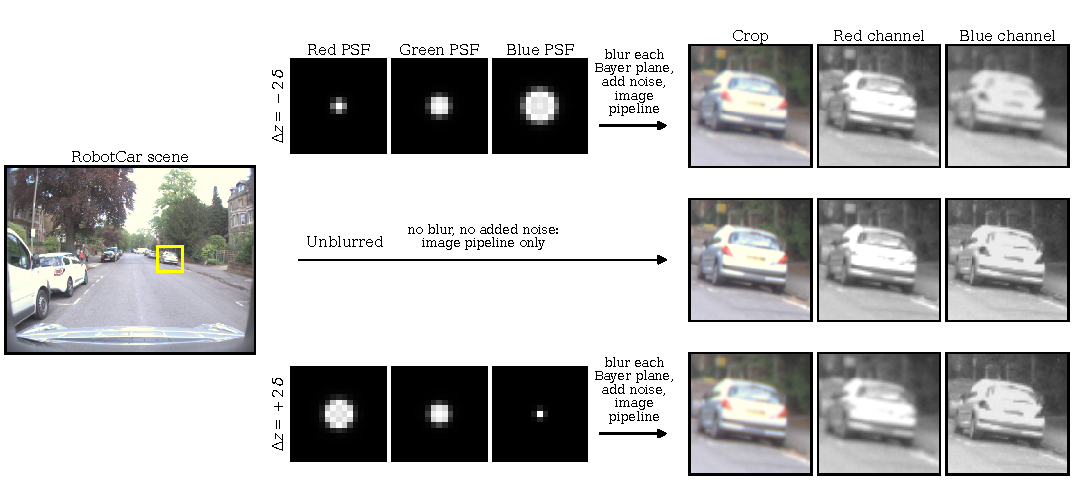
\includegraphics[width=\textwidth]{fig_pipeline.pdf}
\caption{Rendering of one frame. Left: a RobotCar scene, shown rendered in focus, with the cropped region marked. Center: the point-spread function of each color channel for the design with LCA of $2\,\delta$, at displacements of $-2\,\delta$ and $+2\,\delta$. Right: the crop and its red and blue channels. The middle row is the source image passed through the image pipeline with no blur and no added noise. Red is the sharper channel at negative displacement and blue at positive displacement; the chromatic cue measures this difference.}\label{fig:pipeline}\end{figure*}
\begin{figure}[t]\centering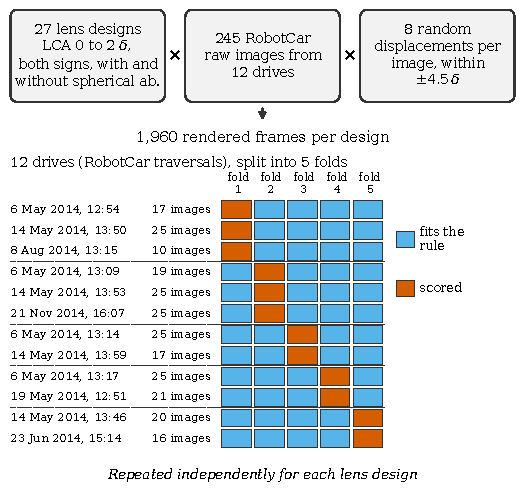
\includegraphics[width=\columnwidth]{fig_design.pdf}
\caption{Design of the rendered experiment. Each lens design is rendered on every RobotCar source image at eight random displacements. The traversals (separate recorded drives, labeled by start time) are split into five groups (folds). In each of five test rounds, one group's drives are scored with the direction threshold $c_0$, sign $s$ and through-focus curve $\gamma$ calibrated on the drives of the other four groups, so a drive is never split between calibration and test.}\label{fig:design}\end{figure}

For comparison on the same rendered frames and traversal folds, we also evaluate two unsigned sharpness baselines (one-dimensional curves against $|\Delta z|$ using frame-median mean green gradient magnitude $\bar\ell$ and finest-band Laplacian-pyramid energy) and a learned gradient-boosted decision-tree regressor \cite{friedman2001greedy} trained on a 69-feature patch summary (per-channel gradient/Tenengrad moments, multi-scale Laplacian-pyramid energies, radial high-frequency spectral power, edge-anisotropy statistics, and cross-channel sharpness ratios, pooled by frame median).

\subsection{PHYSICAL LABORATORY SWEEP}
The laboratory sweep uses a VS Technology VS-0618H1 lens (6\,mm, C-mount) at approximately f/2 on a FLIR Blackfly S BFS-U3-89S6C color camera, with 80 equal servo steps over a 90$^\circ$ focus-ring rotation and an ISO~12233 \cite{iso12233_2023} enhanced spatial frequency response (eSFR) chart at approximately 30\,cm (Fig.~\ref{fig:setup}).
\begin{figure}[t]\centering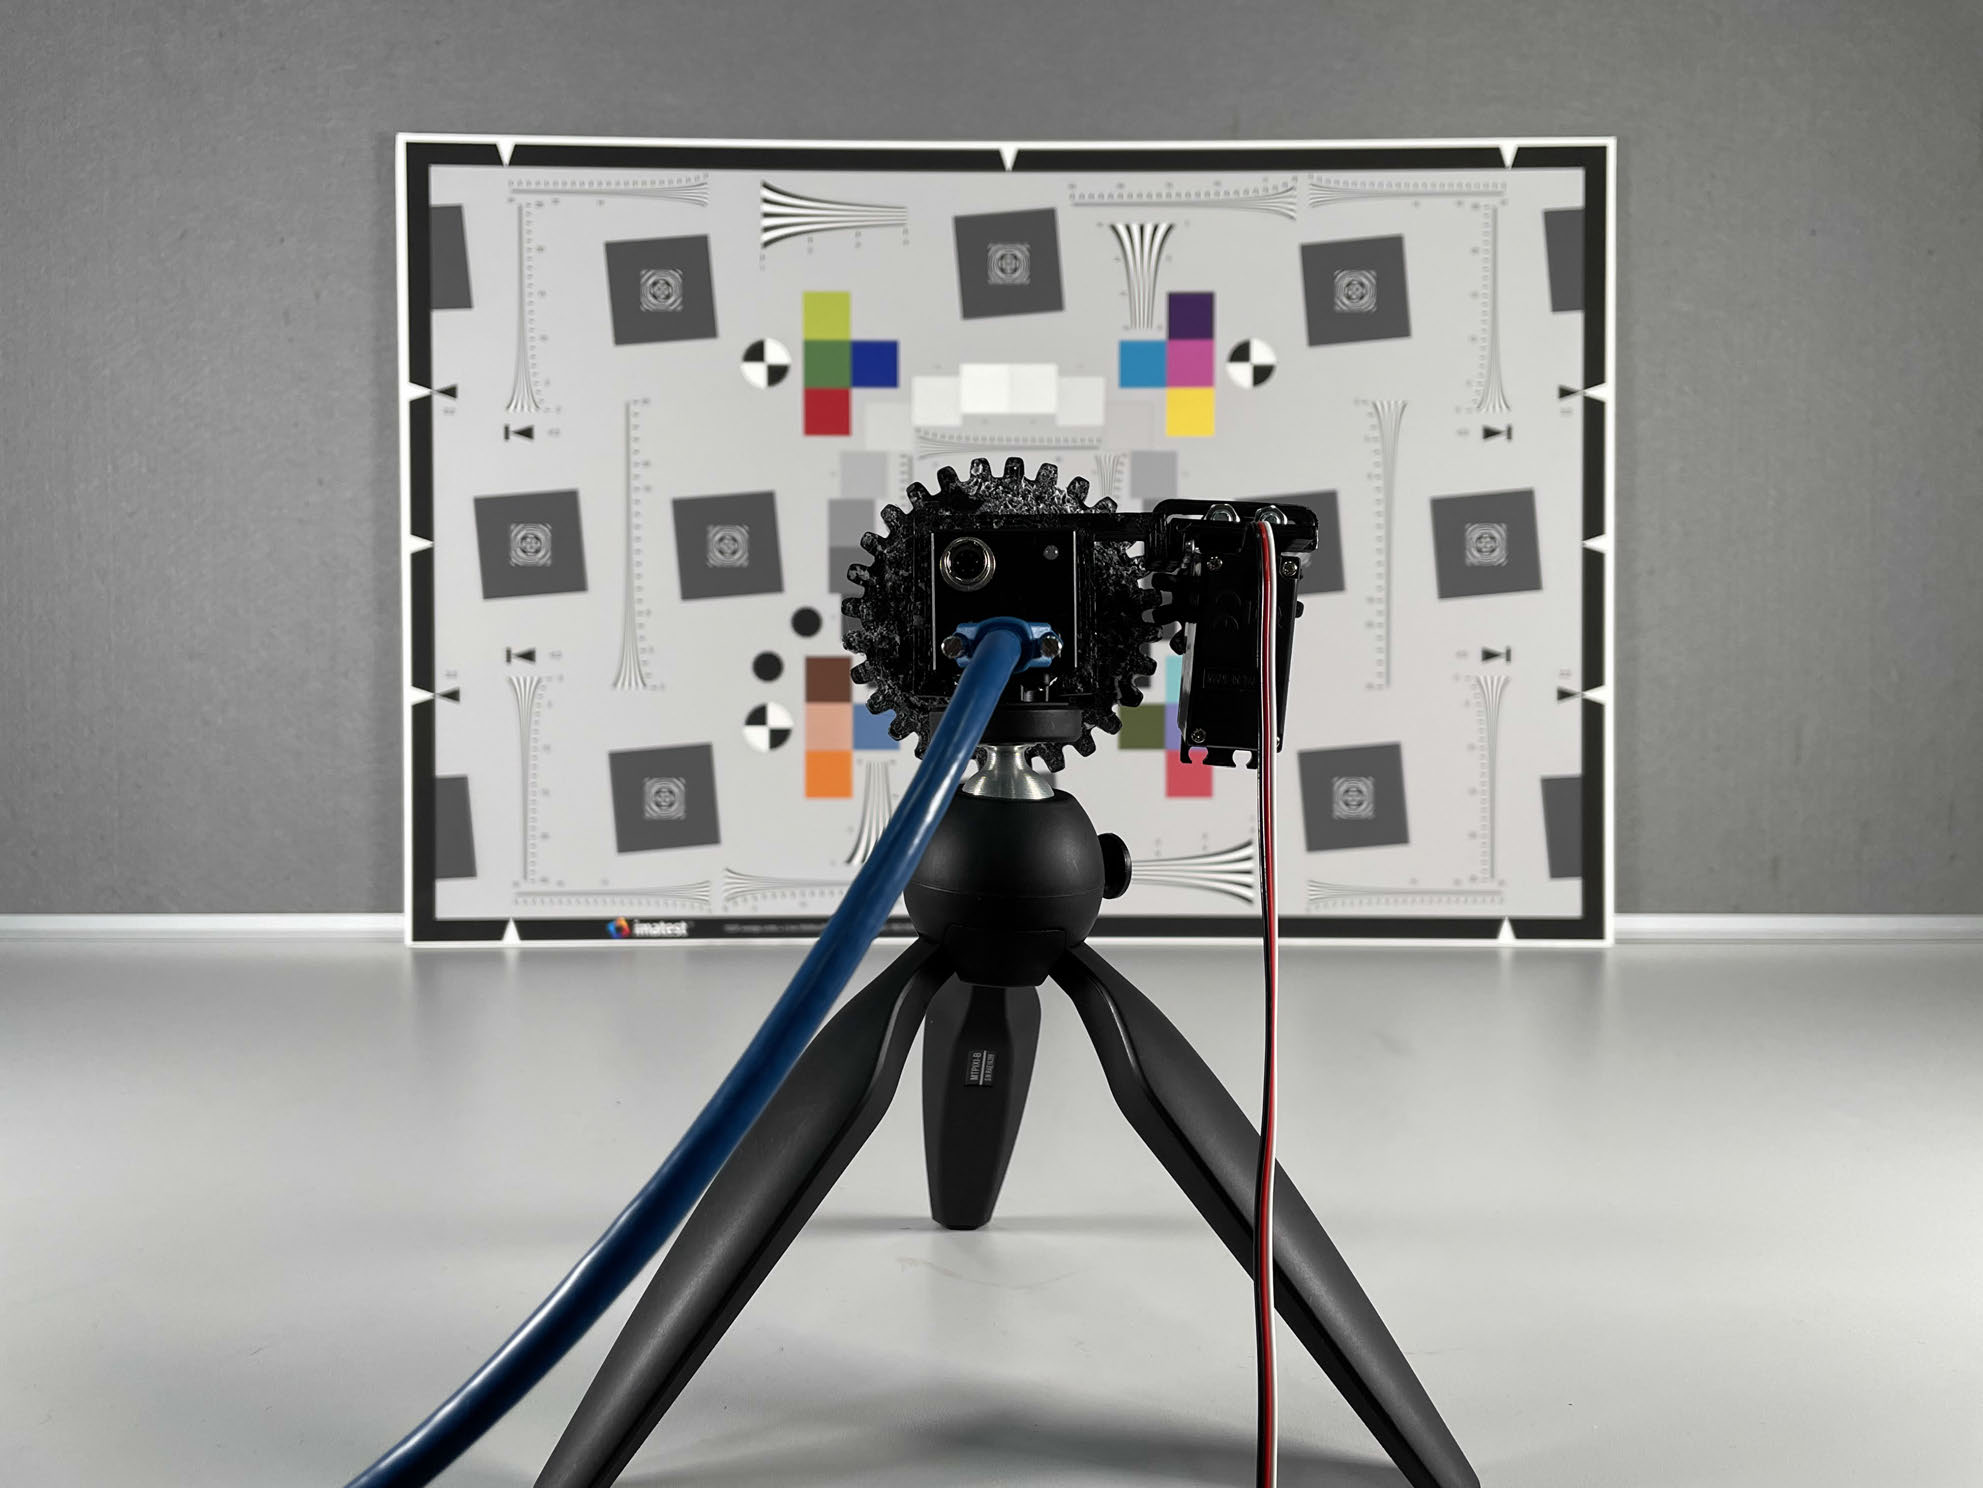
\includegraphics[width=\columnwidth]{fig_lab_setup.jpg}
\caption{Laboratory setup: the camera and lens face the eSFR chart, and a servo turns the lens focus ring through a 3D-printed gear. Reproduced from \cite{deegan2024demosaic}. \note{Placeholder cropped from the earlier paper; replace with an original photograph.}}\label{fig:setup}\end{figure}
The slanted-edge modulation transfer function (MTF), or spatial frequency response (SFR), was measured on the raw Bayer planes \cite{deegan2024demosaic}.
The aperture was set manually to approximately f/2. The sensor pitch, \LabPitchUm\,\textmu m, is taken from the rig record and was not independently verified; with it, $\delta=\LabDeltaUm$\,\textmu m at f/\LabFnum. An exact defocus-OTF fit to the per-channel through-focus MTF yields \LabStepUm\,\textmu m per step at f/\LabFnum{} (residual-bootstrap 95\,\% interval \LabStepCiLo--\LabStepCiHi), corresponding to \LabDeltaPerStep\,$\delta$ per step independent of the f-number, and a red--blue LCA of \LabLcaDelta\,$\delta$ (Fig.~\ref{fig:lab}). Across \LabNvariants{} fit variants (frame subsets, frequencies, and one or three step scales), the step size ranges over \LabDeltaPerStepMin--\LabDeltaPerStepMax\,$\delta$ and the LCA over \LabLcaMin--\LabLcaMax\,$\delta$; LCA is the least precisely constrained laboratory parameter.
The laboratory sweep is partitioned into calibration (every fourth step, left chart half) and test (the remaining steps, right chart half) splits; the test split is evaluated once, after the method is frozen.
\begin{figure*}[t]\centering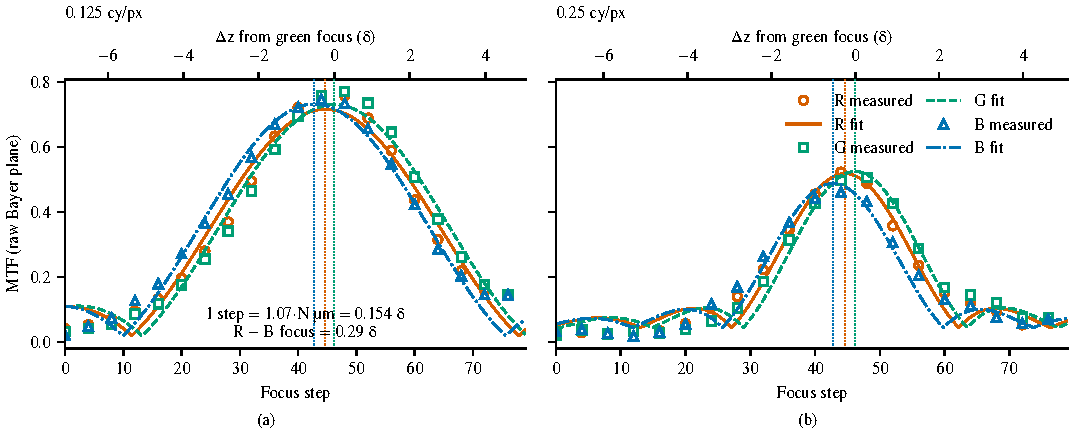
\includegraphics[width=\textwidth]{fig2_lab_through_focus.pdf}
\caption{Laboratory sweep, calibration steps only: raw-Bayer SFR per channel with the exact defocus-OTF fit.}\label{fig:lab}\end{figure*}
To establish the simulation-based prediction for the laboratory lens, we also rendered a matched synthetic design with a red--blue LCA of \LabLcaDelta\,$\delta$ and the green focus plane beyond both, on the same source images, displacements and folds. The per-channel focus offsets are copied from the laboratory fit in units of $\delta$ and mirrored along the focus axis; mirrored pairs of rendered designs yield equivalent performance. This simulation was scored before the laboratory test split was evaluated.

\subsection{FIELD-POSITION AND IN-SERVICE CONFOUND TESTS}
The field-position and in-service confound tests use a discrete nine-rung displacement ladder, $\mathrm{DZ}\in\{0,\pm0.01,\pm0.02,\pm0.05,\pm0.1\}$, where DZ is the renderer's nominal defocus parameter: calibration uses the ladder frames of the training traversals and evaluation scores the same rungs on the held-out traversals. For the synthetic designs 1\,DZ corresponds to 1\,mm of sensor displacement, so 0.01\,DZ equals 10\,\textmu m or $0.45\,\delta$. The ray-traced real lens prescription used in the field-position test (Sony) lacks a recorded f-number and pixel pitch, so its results remain in DZ and cannot be converted to \textmu m or $\delta$. Because these tests are simulations on the discrete ladder rather than the continuous protocol, their errors are not directly comparable with the continuous-displacement results: on the same strong-LCA design ($\SynthLcapLca\,\delta$) the nominal ladder mean absolute error (MAE) is \MsixMaeNominal\,$\delta$, compared with \MtwoMaeDelta\,$\delta$ at continuous displacements. The confound tests compare the strong-LCA design (f/2.0, 5.5\,\textmu m pixel, LCA $\SynthLcapLca\,\delta$) against the laboratory-matched design (f/2.0, 5.5\,\textmu m pixel, LCA $\LabLcaDelta\,\delta$). The confounds are applied to in-focus frames at a strength matched in 90th-percentile gradient sharpness to a $+0.02$\,DZ defocus ($\MeightMatchDelta\,\delta$ on both designs). Motion blur is modeled as an achromatic linear kernel (2.03\,px at $20^\circ$) convolved with each channel's in-focus optical PSF ($\Delta z=0$), preserving the lens's in-focus chromatic signature; this represents uniform translational motion and omits depth-dependent parallax and independent object motion. Fog is modeled as a spatially uniform veiling-airlight layer applied to the raw Bayer image ahead of the in-focus PSF (black level $0$\,DN), $I_{\mathrm{fog},k}=\operatorname{clip}(tI_{\mathrm{raw},k}+A_k(1-t),\,0,\,255)$ with $t=0.956$ and per-plane airlight $A_k$ scaled by the inverse white-balance gain ($A_g=220$\,DN, $A_r=A_g/g_r$, $A_b=A_g/g_b$) so the veil is neutral after white balance, followed by recomputed gray-world white balance; this isolates achromatic contrast reduction and does not model depth-graded extinction, wavelength-dependent scattering or forward-scatter PSF broadening. Fig.~\ref{fig:confound_examples} illustrates the four conditions on one cropped RobotCar region.
\begin{figure*}[t]\centering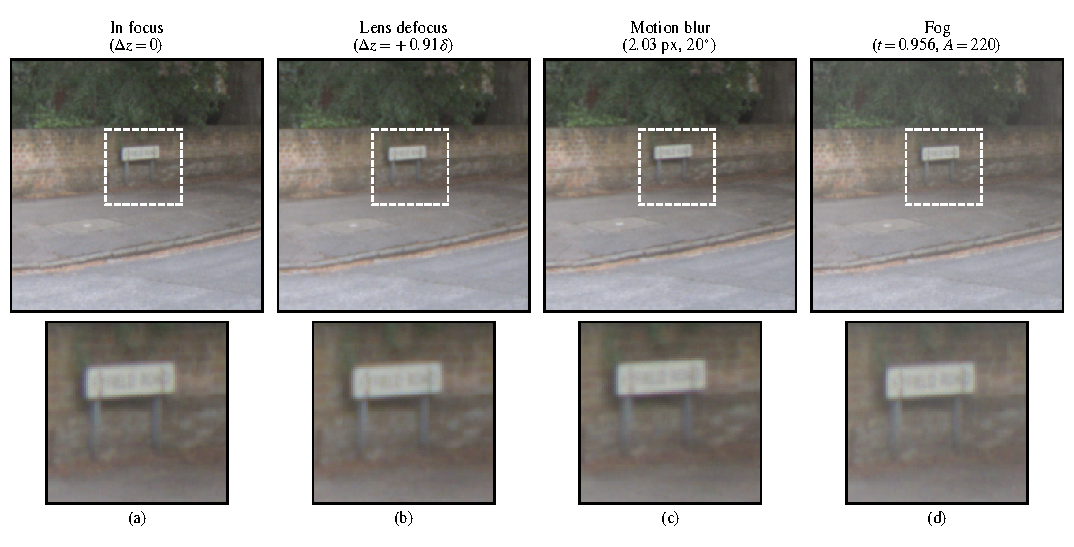
\includegraphics[width=\textwidth]{fig_confound_examples.pdf}
\caption{Qualitative comparison of the four conditions on one $320\times320$-pixel RobotCar crop (strong-LCA design, $\SynthLcapLca\,\delta$), with a $3.3\times$ zoom of the dashed $96\times96$-pixel sign region below each panel: (a)~in-focus baseline ($\Delta z=0$), (b)~lens defocus ($\Delta z=+\MeightMatchDelta\,\delta$), (c)~in-focus linear motion blur (2.03\,px at $20^\circ$, convolved with the in-focus optical PSF), and (d)~in-focus neutral uniform fog ($t=0.956$, $A_g=220$\,DN, inverse-white-balance scaled). Motion blur and fog are calibrated to match the 90th-percentile gradient sharpness loss of (b).}\label{fig:confound_examples}\end{figure*}

\subsection{METRICS AND PRE-SPECIFIED CRITERIA}
We score each frame $i$ of a test set by the error $e_i=\widehat{\Delta z}_i-\Delta z_i$ in units of $\delta$. Over the set $\mathcal{F}$ of frames that return an estimate,
\begin{equation}
\mathrm{MAE}=\frac{1}{|\mathcal{F}|}\sum_{i\in\mathcal{F}}|e_i|,\qquad
\mathrm{bias}=\frac{1}{|\mathcal{F}|}\sum_{i\in\mathcal{F}}e_i ,
\end{equation}
and p90 is the 90th percentile of $|e_i|$ over $\mathcal{F}$. Direction accuracy is
\begin{equation}
\mathrm{acc}=\frac{1}{|\mathcal{F}_d|}\sum_{i\in\mathcal{F}_d}\mathbf{1}\bigl[\hat d_i=\operatorname{sign}\Delta z_i\bigr],
\end{equation}
where $\mathcal{F}_d\subseteq\mathcal{F}$ excludes frames without a defined direction: rendered displacements are continuous and never zero, whereas in the laboratory sweep a frame within half a step of best focus has no ground-truth direction and is excluded. The abstention rate is the fraction of frames returning no estimate; abstentions are excluded from $\mathcal{F}$ and reported separately. Laboratory results are reported as counts without confidence intervals because the frames are consecutive steps of a single sweep and are not independent. Confidence intervals on rendered results resample whole traversals, the 12 drives (2000 bootstrap draws), and we also report the range across the five folds. For the in-service tests a frame raises an \emph{alarm} when $|\widehat{\Delta z}|>\tau_{\mathrm{alarm}}$, where $\tau_{\mathrm{alarm}}$ is the 95th percentile of $|\widehat{\Delta z}|$ over the in-focus ($\Delta z=0$) training frames of the same fold, predicted with that fold's calibration. Because $\tau_{\mathrm{alarm}}$ is determined from training frames only, the in-focus alarm rate on test frames is measured rather than fixed at 5\,\%.

Two success criteria were pre-specified prior to experimentation. First, the direction-trend criterion requires direction accuracy to increase monotonically with LCA/$\delta$ across the lens population (Spearman $\rho>0$, one-sided $p<0.05$). Second, the displacement-accuracy criterion requires the mean absolute displacement error on displacements absent from training to remain below $1\,\delta$ for designs with $|\mathrm{LCA}|>1\,\delta$. Failure to meet the direction-trend criterion would falsify the central hypothesis; failure to meet the displacement-accuracy criterion would restrict the claim to sign estimation.
Nine deviations from the pre-specified protocol occurred during execution and are documented in the Appendix.

\section{RESULTS}
Table~\ref{tab:req} summarizes the four requirements; the following subsections present the supporting evidence for each.
\begin{table*}[t]\centering\footnotesize
\caption{The four requirements, the principal finding for each, and the supporting evidence (distinguishing pre-specified confirmatory tests from post-freeze exploratory analyses). Direction: fraction of frames with the correct sign. The alarm criterion is defined in Section~\ref{sec:design}.}
\label{tab:req}
\begin{tabular}{p{0.20\textwidth}p{0.50\textwidth}p{0.22\textwidth}}\toprule
Requirement & Finding & Evidence \\\midrule
Sufficient LCA, approximately $1\,\delta$ (for frozen baseline over $\pm\MthreeDzMaxDelta\,\delta$) & Direction accuracy \MthreeLvlZeroDirMin--\MthreeLvlZeroDirMax{} at zero LCA, \MthreeLvlHalfDirMin--\MthreeLvlHalfDirMax{} at $0.5\,\delta$, \MthreeLvlOneDirMin--\MthreeLvlOneDirMax{} at $1\,\delta$ (\MthreeLvlOneNearMin--\MthreeLvlOneNearMax{} within $0.5\,\delta$ of focus) & Rendered, \MthreeNlenses{} lens designs (pre-specified) \\
Stronger magnitude estimation & Error in $|\Delta z|$: learned regressor \RefLearnAbsMin--\RefLearnAbsMax\,$\delta$, Laplacian metric \RefLapAbsMin--\RefLapAbsMax\,$\delta$ (exploratory pairing \RefPairedMaeMin--\RefPairedMaeMax\,$\delta$ signed MAE), two-feature curve \RefPhysAbsMin--\RefPhysAbsMax\,$\delta$ & Rendered, designs above $1\,\delta$ (reference + exploratory) \\
Camera-specific calibration & Rendered-only calibration predicts one sign for all frames. Empirical threshold: \LabBandFarOk{} of \LabBandFarN{} beyond $2\,\delta$, \LabBandNearOk{} of \LabBandNearN{} within $2\,\delta$ (pre-specified); fails across chart halves (exploratory) & One physical lens, one static sweep, single held-out evaluation \\
Rejection of non-defocus degradations & Pooled single-frame alarm rate: in-focus \MeightStrongPooledInFocus, motion \MeightStrongPooledMotion, fog \MeightStrongPooledFog{} vs.\ defocus \MeightStrongPooledDefPos; 100-frame averaging raises fog to \MeightAggStrongHundredFog{} and motion to \MeightAggStrongHundredMotion & Simulation, strong-LCA design \\\bottomrule
\end{tabular}
\end{table*}

\subsection{MINIMUM LCA REQUIREMENT}\label{sec:req1}
For the frozen two-feature estimator over $\pm\MthreeDzMaxDelta\,\delta$, direction accuracy is near chance without LCA and saturates at approximately $1\,\delta$.
Each of the \MthreeNlenses{} designs is rendered on \MthreeNframes{} frames (every RobotCar source image at eight continuous displacements). Over the designs at each LCA level (both signs, with and without SA), direction accuracy is \MthreeLvlZeroDirMin--\MthreeLvlZeroDirMax{} at $0$, \MthreeLvlQuarterDirMin--\MthreeLvlQuarterDirMax{} at $0.25$, \MthreeLvlHalfDirMin--\MthreeLvlHalfDirMax{} at $0.5$, \MthreeLvlThreeQDirMin--\MthreeLvlThreeQDirMax{} at $0.75$, \MthreeLvlOneDirMin--\MthreeLvlOneDirMax{} at $1$, \MthreeLvlOneHalfDirMin--\MthreeLvlOneHalfDirMax{} at $1.5$ and \MthreeLvlTwoDirMin--\MthreeLvlTwoDirMax{} at $2\,\delta$ (Fig.~\ref{fig:m3}). The \MthreeLevelN{} level means increase monotonically (Spearman $\rho=\MthreeLevelRho$, exact one-sided permutation $p=\MthreeLevelP$). Across individual designs, Spearman $\rho=\MthreeRho$ and Kendall $\tau=\MthreeTau$, with one-sided $p=\MthreeGateAP$ ($n=\MthreeNlenses$), satisfying the pre-specified direction-trend criterion. At zero LCA, direction accuracy is near chance: \MthreeZeroDir{} (95\,\% interval \MthreeZeroDirLo--\MthreeZeroDirHi) without and \MthreeZeroSaDir{} (\MthreeZeroSaDirLo--\MthreeZeroSaDirHi) with SA, and at $0.25\,\delta$ it is \MthreeQuarterDirMin--\MthreeQuarterDirMax.

This approximately $1\,\delta$ knee is conditional on the uniform $\pm\MthreeDzMaxDelta\,\delta$ displacement distribution, the red--blue LCA definition, and the frozen two-feature estimator. Broken down by distance from focus, designs at $|\mathrm{LCA}|=1\,\delta$ reach \MthreeLvlOneMidMin--\MthreeLvlOneMidMax{} direction accuracy for $|\Delta z|\in[0.5,1)\,\delta$ and $0.98$--$1.00$ beyond $1\,\delta$, whereas within $0.5\,\delta$ of focus accuracy is only \MthreeLvlOneNearMin--\MthreeLvlOneNearMax{} (rising to \MthreeLvlTwoNearMin--\MthreeLvlTwoNearMax{} at $2\,\delta$). Moreover, as Section~\ref{sec:req2} shows, a learned multi-feature regressor trained per lens reaches \RefHalfLearnDirMin--\RefHalfLearnDirMax{} overall direction accuracy already at $0.5\,\delta$ LCA.
The laboratory lens, at \LabLcaDelta\,$\delta$, lies in the low-accuracy region of this curve; Section~\ref{sec:req3} evaluates it.
\begin{figure*}[t]\centering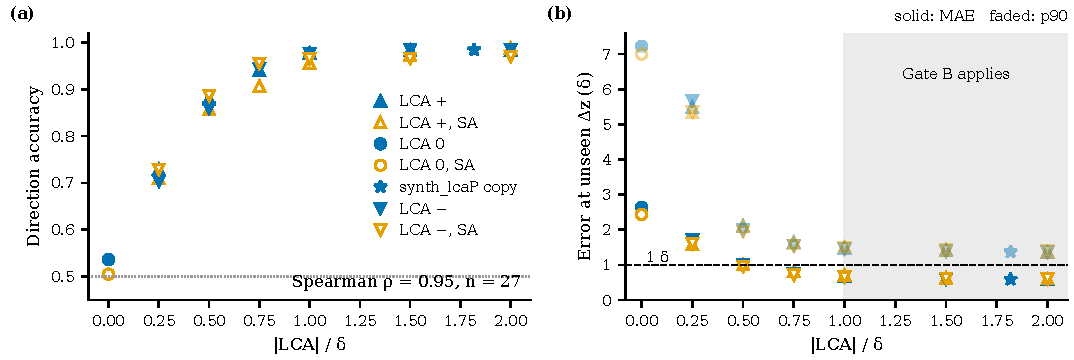
\includegraphics[width=\textwidth]{fig1_m3_dose_response.pdf}
\caption{Direction and error against LCA, \MthreeNlenses{} rendered lens designs. (a) Direction accuracy against $|\mathrm{LCA}|/\delta$. (b) MAE and p90 on the \MthreeUnseenN{} test frames per design whose continuous displacement is absent from training; the shaded region marks $|\mathrm{LCA}|>1\,\delta$, where the $\mathrm{MAE}<1\,\delta$ criterion applies.}\label{fig:m3}\end{figure*}

\subsection{STRONGER MAGNITUDE ESTIMATION}\label{sec:req2}
With sufficient LCA, the frozen two-feature estimator satisfies the pre-specified displacement criterion; however, its magnitude accuracy is limited by its mean-gradient-magnitude sharpness feature, and both finest-band Laplacian energy and learned multi-feature regression improve it substantially.
Test displacements are continuous and test drives are held out. Because each frame's displacement is drawn independently, a test displacement rounded to 0.1\,\textmu m can also occur in another fold's training frames; the displacement-accuracy criterion is therefore scored on the \MthreeUnseenN{} of \MthreeNframes{} test frames per design whose rounded displacement occurs in no training fold. For the \MthreeGateBN{} designs with $|\mathrm{LCA}|>1\,\delta$, MAE on these frames is \MthreeGateBMaeMin--\MthreeGateBMaeMax\,$\delta$, satisfying the $\mathrm{MAE}<1\,\delta$ criterion; on all test frames it is \MthreeGateBMaeAllMin--\MthreeGateBMaeAllMax\,$\delta$, and over all \MthreeNlenses{} designs the two differ by at most \MthreeUnseenMaxDiff\,$\delta$. At $0.25\,\delta$ the MAE on displacements absent from training is \MthreeQuarterMaeMin--\MthreeQuarterMaeMax\,$\delta$. Across the \MthreeGateBN{} designs with $|\mathrm{LCA}|>1\,\delta$, the upper bounds of the traversal-clustered 95\,\% confidence intervals for unseen-displacement MAE reach at most \MthreeGateBCiHiMax\,$\delta$, and the worst single fold reaches \MthreeGateBFoldMax\,$\delta$. The remaining results in this subsection use all test frames. For the strong-LCA reference design ($\SynthLcapLca\,\delta$, Fig.~\ref{fig:m2}), MAE is \MtwoMaeDelta\,$\delta$ (95\,\% interval \MtwoMaeCiLo--\MtwoMaeCiHi; \MtwoMaeUm\,\textmu m) and p90 \MtwoPninetyDelta\,$\delta$, and direction accuracy is \MtwoDirAll{} overall and \MtwoDirNear{} within $0.5\,\delta$ of focus. On a separate \MtwoSubsetN-frame render of the same design (not a subset of these frames), training on the nine-rung ladder instead of continuous displacements yields equivalent error (\MtwoSubsetLadderMaeDelta{} against \MtwoSubsetMaeDelta\,$\delta$).
\begin{figure*}[t]\centering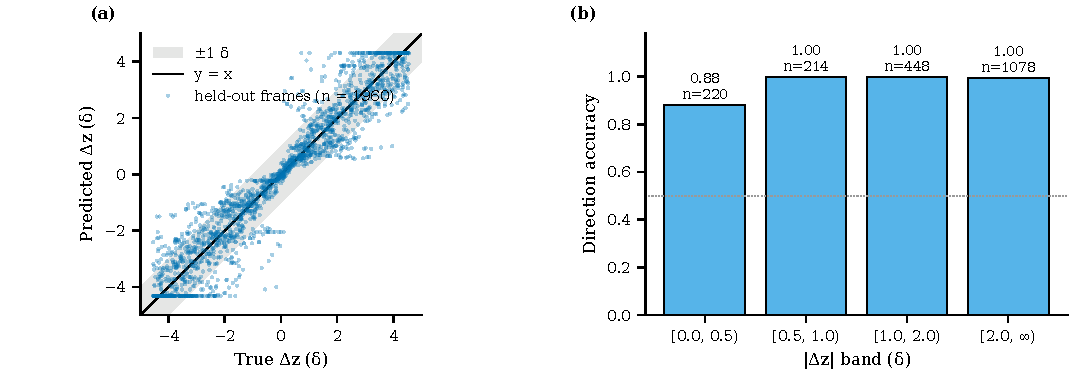
\includegraphics[width=\textwidth]{fig3_m2_continuous.pdf}
\caption{Strong-LCA reference design ($\SynthLcapLca\,\delta$), \MtwoN{} held-out frames at continuous displacements. (a) Predicted against true $\Delta z$; horizontal bands arise from endpoint saturation at $\pm 4.32\,\delta$ and nearest-point projection onto the 10\,\textmu m polyline bin centers. (b) Direction accuracy per $|\Delta z|$ band.}\label{fig:m2}\end{figure*}

On the same frames and folds, we evaluate the two unsigned sharpness baselines (mean green gradient magnitude and finest-band Laplacian-pyramid energy) and the 69-feature learned gradient-boosting regressor (Table~\ref{tab:ref}).
For magnitude estimation alone, the Laplacian baseline (\RefLapAbsMin--\RefLapAbsMax\,$\delta$) is substantially more accurate than the two-feature curve (\RefPhysAbsMin--\RefPhysAbsMax\,$\delta$) and the mean-gradient-magnitude baseline (\RefTenAbsMin--\RefTenAbsMax\,$\delta$).
Because the two-feature curve derives its magnitude primarily from $\bar\ell$---the same mean-gradient-magnitude feature---its $|\Delta z|$ error closely tracks that baseline (\RefPhysAbsMin--\RefPhysAbsMax{} against \RefTenAbsMin--\RefTenAbsMax\,$\delta$), while the chromatic ratio $\bar c$ supplies the sign. Pairing the two-feature sign with the Laplacian baseline's $|\widehat{\Delta z}|$ was not part of the frozen estimator; evaluated on rendered data only as a post-freeze exploratory analysis (\emph{Paired}, Table~\ref{tab:ref}), it reduces signed MAE for designs above $1\,\delta$ from \RefPhysMaeMin--\RefPhysMaeMax\,$\delta$ to \RefPairedMaeMin--\RefPairedMaeMax\,$\delta$ (and to \RefHalfPairedMae\,$\delta$ at $0.5\,\delta$, where direction accuracy equals the two-feature rule by construction).

The learned 69-feature regressor does not separate sign from magnitude and achieves the lowest error on rendered data: for the \RefGateBN{} designs with $|\mathrm{LCA}|>1\,\delta$, its signed MAE is \RefLearnMaeMin--\RefLearnMaeMax\,$\delta$ and its $|\Delta z|$ error is \RefLearnAbsMin--\RefLearnAbsMax\,$\delta$, outperforming even the Laplacian baseline. At $0.5\,\delta$ LCA it achieves \RefHalfLearnDirMin--\RefHalfLearnDirMax{} direction accuracy (MAE \RefHalfLearnMae\,$\delta$), and at $0.25\,\delta$ it reaches \RefQuarterLearnDirMin--\RefQuarterLearnDirMax{} direction accuracy, though its signed MAE (\RefQuarterLearnMaeMin--\RefQuarterLearnMaeMax\,$\delta$) remains unusable. Thus the rendered results do not prove that sign and magnitude must be estimated separately; rather, they show that if a lightweight, lens-agnostic two-feature rule is used instead of per-lens multi-feature training, replacing mean gradient magnitude with a higher-frequency sharpness metric (Laplacian energy) recovers much of the magnitude gap. All reference methods are trained and tested on renders of a single lens design each; none is evaluated on the held-out laboratory split.
\begin{table}[t]\centering\footnotesize
\caption{Reference rows on the Phase~2 render, designs without spherical aberration, mean over the two LCA signs (designs with it: results/reference). Dir.: direction accuracy, a fraction of frames (two-feature method as in Fig.~\ref{fig:m3}). MAE: error of the signed estimate $\widehat{\Delta z}$; $|\Delta z|$: error of the magnitude only; both in $\delta$.}
\label{tab:ref}\setlength{\tabcolsep}{3pt}
\begin{tabular}{rcccccccc}\toprule
LCA/$\delta$ & \multicolumn{3}{c}{Two-feature} & \multicolumn{3}{c}{Learned} & Laplacian & Tenengrad \\
\cmidrule(lr){2-4}\cmidrule(lr){5-7}\cmidrule(lr){8-8}\cmidrule(lr){9-9}
 & Dir. & MAE & $|\Delta z|$ & Dir. & MAE & $|\Delta z|$ & $|\Delta z|$ & $|\Delta z|$ \\\midrule
0.00 & 0.54 & 2.64 & 0.64 & 0.51 & 2.26 & 2.18 & 0.29 & 0.65 \\
0.25 & 0.72 & 1.65 & 0.66 & 0.86 & 1.82 & 1.74 & 0.29 & 0.65 \\
0.50 & 0.87 & 1.00 & 0.65 & 0.94 & 1.13 & 1.09 & 0.29 & 0.65 \\
0.75 & 0.94 & 0.78 & 0.63 & 0.97 & 0.69 & 0.67 & 0.29 & 0.65 \\
1.00 & 0.98 & 0.67 & 0.62 & 0.98 & 0.45 & 0.45 & 0.29 & 0.65 \\
1.50 & 0.98 & 0.61 & 0.60 & 0.99 & 0.25 & 0.25 & 0.29 & 0.65 \\
2.00 & 0.98 & 0.59 & 0.59 & 0.99 & 0.18 & 0.18 & 0.29 & 0.65 \\
\bottomrule\end{tabular}\end{table}


\subsection{CAMERA-SPECIFIC CALIBRATION AND TRANSFER LIMITS}\label{sec:req3}
The physical lens requires a camera-specific threshold, yields reliable direction estimates only beyond $2\,\delta$ from focus, and exhibits a near-focus cue discrepancy between halves of the test chart.
The laboratory-matched simulation establishes the prior expectation on driving scenes: direction accuracy \MfiveDir{} and displacement MAE \MfiveMae\,$\delta$, intermediate between the rendered designs at $0.25\,\delta$ and $0.5\,\delta$, predicting weak directional sensitivity and unusable displacement accuracy for a $\LabLcaDelta\,\delta$ lens.

On the laboratory calibration split alone (20 steps, left chart half), direction classification is correct on \LabCalDirOk{} of \LabCalDirN{} frames and leave-one-out displacement MAE over \LabCalMaeN{} frames is \LabCalMaeDelta\,$\delta$. The within-frame sampling error of the chromatic cue alone has a median of \MfourSeMedianDelta\,$\delta$ and ranges from \MfourSeMinDelta{} to \MfourSeMaxDelta\,$\delta$; because the sweep contains a single exposure per step, exposure-to-exposure repeatability is not measured.
In an exploratory calibration-split comparison across the \LabSharpCalN{} steps (left chart half only), both unsigned sharpness metrics track raw-Bayer green MTF monotonically on both sides of focus (Fig.~\ref{fig:lab_sharpness_mtf}): Spearman $\rho=\LabTenMtfLowRho$ (mean $|\nabla I_g|$) and $\LabLapMtfLowRho$ (Laplacian) at 0.125\,cycles/pixel, and $\LabTenMtfHighRho$ and $\LabLapMtfHighRho$ at 0.25\,cycles/pixel. However, mean $|\nabla I_g|$ compresses to a far-defocus floor of \LabTenFloorPct\,\% of its peak whereas Laplacian-pyramid energy drops to \LabLapFloorPct\,\% of its peak and follows high-frequency MTF more closely, corroborating on physical hardware why Laplacian energy outperforms mean $|\nabla I_g|$ for magnitude estimation in Table~\ref{tab:ref}; this comparison is restricted to the calibration split and does not alter or re-score the frozen held-out test split.
\begin{figure}[t]\centering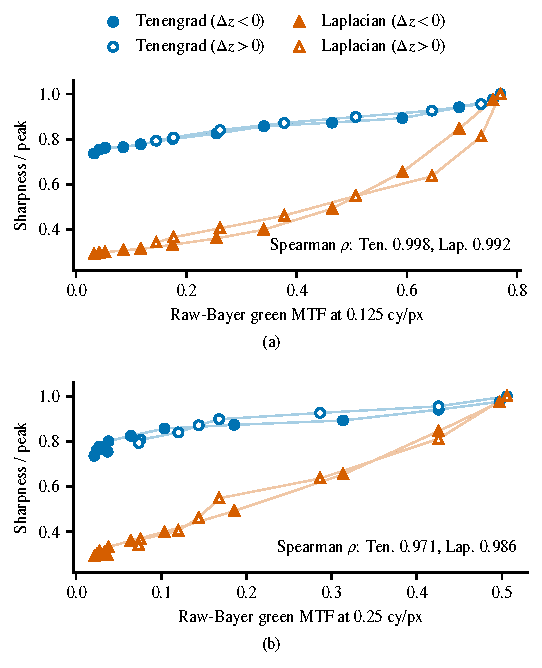
\includegraphics[width=\columnwidth]{fig_lab_sharpness_mtf.pdf}
\caption{Exploratory laboratory calibration-split comparison (\LabSharpCalN{} steps, left chart half only): peak-normalized mean green gradient magnitude ($|\nabla I_g|$) and finest-band Laplacian-pyramid energy against raw-Bayer green MTF at (a) 0.125 and (b) 0.25\,cycles/pixel. Filled and open markers denote negative and positive defocus relative to fitted green best focus; both sides collapse onto one monotonic curve, illustrating the sign ambiguity of unsigned sharpness.}\label{fig:lab_sharpness_mtf}\end{figure}

On the held-out test split (right chart half, the remaining \LabTestNsteps{} of 80 steps), evaluated once with the method frozen, \LabTestCalN{} frames have a defined direction (the remaining step lies within half a step of green focus), \LabTestNegN{} of which are on the negative side. Calibration from rendered data alone predicts negative defocus on every frame, so its \LabTestRenderedOk{} of \LabTestRenderedN{} equals the majority-class rate; its displacement MAE is \LabTestRenderedMae\,$\delta$. Using the measured channel order with a threshold from the calibration split yields \LabTestOrderOk{} of \LabTestOrderN{}. Full calibration produces the same sign and threshold, so its direction rule is identical and the equal count does not constitute independent evidence; its displacement MAE is \LabTestCalMae\,$\delta$ with a signed bias of \LabTestCalBias\,$\delta$. Accuracy depends strongly on distance from focus. Beyond $2\,\delta$, direction is correct on \LabBandFarOk{} of \LabBandFarN{} frames (majority class \LabBandFarMaj) and MAE is \LabTestFarMae\,$\delta$; because this is a single static sweep of one chart, this result shows consistency with the calibrated rule far from focus without isolating LCA as the sole mechanism. Within $2\,\delta$ it is correct on \LabBandNearOk{} of \LabBandNearN{} (majority class \LabBandNearMaj), and within $3\,\delta$ on \LabBandNearThreeOk{} of \LabBandNearThreeN{} (majority class \LabBandNearThreeMaj): near focus the calibrated rule performs no better than majority-class prediction. Because the frames are consecutive steps of a single static sweep rather than independent observations, we report counts without binomial confidence intervals; they characterize this sweep rather than a population of scenes or lenses.

In a post-hoc exploratory analysis, we applied the same frozen rule to the two laboratory subsets that vary only one factor; neither overlaps the test split.
On the left half at the non-calibration steps (steps vary, chart half fixed), direction is correct on \LabTrStepsAllOk{} of \LabTrStepsAllN{} frames (\LabTrStepsNearOk{} of \LabTrStepsNearN{} within $2\,\delta$) and MAE is \LabTrStepsMae\,$\delta$.
On the right half at the calibration steps (chart half varies, steps fixed), it is \LabTrHalfAllOk{} of \LabTrHalfAllN{} (\LabTrHalfNearOk{} of \LabTrHalfNearN{} within $2\,\delta$) and MAE is \LabTrHalfMae\,$\delta$.
Within $2\,\delta$ of focus the chromatic cue differs by a median of \LabTrOffsetNear{} on the right half relative to the left at the same steps, compared with \LabTrOffsetAll{} across the full sweep; near focus the right-half cue also loses monotonic separation across zero rather than shifting by a simple constant threshold offset.
The near-focus failure therefore tracks the change of chart half rather than interpolation between calibration steps; because the sweep images a single static scene, these counts are not independent samples.

Spatial field position degrades directional accuracy in simulation as well.
Under the full field-varying PSF of the Sony design, direction accuracy falls from \MsevenUniMidDir{} to \MsevenFvMidDir{} in the mid zone and to \MsevenFvCornerDir{} in the corner; against each zone's own best focus it is \MsevenFvMidDirLocal{} and \MsevenFvCornerDirLocal. A center calibration leaves an off-axis bias of \MsevenFvMidBias\,DZ; per-zone calibration removes it (\MsevenZcMidBias\,DZ) but does not restore direction accuracy (\MsevenZcMidDir{} mid, \MsevenZcCornerDir{} corner). On the laboratory chart squares at 0.25\,cycles/pixel (exploratory), the red$-$blue best-focus difference is \MsevenLabCenter\,$\delta$ at the center, but its median changes sign in the mid (\MsevenLabMid\,$\delta$) and corner (\MsevenLabCorner\,$\delta$) zones.

\subsection{REJECTION OF NON-DEFOCUS DEGRADATIONS}\label{sec:req4}
In simulation, in-focus motion blur and fog trigger false defocus alarms, and multi-frame averaging amplifies them; illuminant shifts and white-balance errors bias the displacement magnitude without changing its sign.
On the strong-LCA design ($\SynthLcapLca\,\delta$), in-focus motion blur and fog raise the per-fold training-threshold alarm rate from \MeightStrongInFocus{} to \MeightStrongMotion{} and \MeightStrongFog, against \MeightStrongDefocusNeg{} and \MeightStrongDefocusPos{} for a real defocus of $-0.02$ and $+0.02$\,DZ ($\pm\MeightMatchDelta\,\delta$). However, the per-fold training threshold $\tau_{\mathrm{alarm}}$ varies sevenfold across the five folds (\MeightStrongThrMinDelta--\MeightStrongThrMaxDelta\,$\delta$) because the 95th percentile is estimated from approximately 190 quantized in-focus predictions on the finite inversion grid, so the single-frame defocus alarm rate swings from \MeightStrongDefFoldMin{} to \MeightStrongDefFoldMax{} across folds (reflected in the wide drive-bootstrap intervals of Fig.~\ref{fig:m8}(a)). Evaluated at a single pooled held-out threshold (the 95th percentile of held-out in-focus $|\widehat{\Delta z}|$), single-frame separation is weak: defocus alarms on \MeightStrongPooledDefNeg{} ($-0.02$\,DZ) and \MeightStrongPooledDefPos{} ($+0.02$\,DZ), against \MeightStrongPooledInFocus{} in focus, \MeightStrongPooledMotion{} under motion blur, and \MeightStrongPooledFog{} under fog. On the laboratory-matched design ($\LabLcaDelta\,\delta$), motion blur (\MeightWeakMotion) and fog (\MeightWeakFog) alarm at rates comparable to or exceeding real defocus (\MeightWeakDefocusNeg{} at $-0.02$ and \MeightWeakDefocusPos{} at $+0.02$\,DZ; Fig.~\ref{fig:m8}).
\begin{figure*}[t]\centering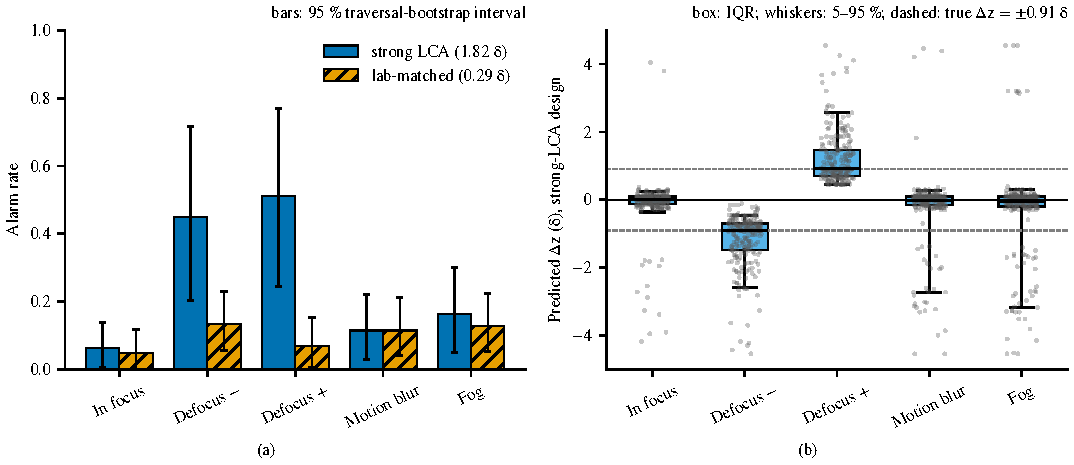
\includegraphics[width=\textwidth]{fig5_m8_confounds.pdf}
\caption{Effect of in-focus motion blur and fog compared with true defocus ($\Delta z=\pm\MeightMatchDelta\,\delta$, labeled Defocus~$-$ and Defocus~$+$) for the strong-LCA design ($\SynthLcapLca\,\delta$) and the laboratory-matched design ($\LabLcaDelta\,\delta$). Motion blur (2.03\,px at $20^\circ$, convolved with the in-focus optical PSF) and neutral fog ($t=0.956$, $A_g=220$\,DN) are calibrated to match the sharpness loss of $+\MeightMatchDelta\,\delta$ defocus. (a)~Single-frame defocus alarm rate, defined as the fraction of frames whose predicted $|\widehat{\Delta z}|$ exceeds the 95th percentile of training-fold in-focus predictions; error bars show 95\,\% confidence intervals obtained by resampling whole drives (wide intervals on the strong-LCA design reflect fold-to-fold threshold spread). (b)~Per-frame predicted displacement $\widehat{\Delta z}$ on the strong-LCA design (gray points), with boxes showing the interquartile range (IQR), center bars the median, whiskers the 5th--95th percentiles, and dashed lines the true $\pm\MeightMatchDelta\,\delta$ defocus levels.}\label{fig:m8}\end{figure*}

As a detector of defocus against in-focus frames, $|\widehat{\Delta z}|$ has receiver operating characteristic area under the curve (ROC AUC) \MeightAucStrongFocusMin--\MeightAucStrongFocusMax{} on the strong-LCA design and \MeightAucWeakFocusMin--\MeightAucWeakFocusMax{} on the laboratory-matched design; against motion blur it is \MeightAucStrongMotionMin--\MeightAucStrongMotionMax{} and \MeightAucWeakMotionMin--\MeightAucWeakMotionMax, and against fog \MeightAucStrongFogMin--\MeightAucStrongFogMax{} and \MeightAucWeakFogMin--\MeightAucWeakFogMax{} (near chance on the laboratory-matched design). A fleet deployment would typically average estimates across multiple frames. Evaluating bootstrap windows of $N$ frames drawn with replacement from one condition's held-out frames, with the alarm threshold at the 95th percentile of held-out in-focus averages (drawn from the same in-focus pool), the strong-LCA design alarms on all defocused windows from $N=10$, whereas fog alarms on \MeightAggStrongTenFog{} at $N=10$ and \MeightAggStrongHundredFog{} at $N=100$, and motion blur alarms on \MeightAggStrongTenMotion{} at $N=10$ and \MeightAggStrongHundredMotion{} at $N=100$ (against \MeightAggStrongHundredFocus{} in focus) because reduced sharpness pushes outlier frames onto the negative defocus branch (Fig.~\ref{fig:m8}(b)) and shifts the window mean. For $N=1$ this pooled bootstrap threshold gives single-frame defocus alarm rates of \MeightAggStrongOneDefocus--\MeightAggStrongOneDefocusMax, close to the direct pooled rate above (differing slightly due to ties on the quantized inversion grid). On the laboratory-matched design, 100-frame averaging raises the defocus alarm rate to \MeightAggWeakHundredDefocus--\MeightAggWeakHundredDefocusMax{}, while driving fog to \MeightAggWeakHundredFog{} (motion blur stays at \MeightAggWeakHundredMotion{} because its mean predicted displacement lies near zero on this design). Without separate screening to reject motion blur and fog, temporal averaging therefore amplifies confounding degradations alongside the defocus signal. Because frames within a real drive are temporally correlated rather than independent bootstrap draws, both signal accumulation and confound accumulation will be slower in practice, and each window is assumed to hold one condition throughout.

On the strong-LCA design, illuminant shifts of $\pm10$\,nm bias the displacement by at most \MsixShiftBiasMax\,$\delta$, and white-balance errors raise MAE from \MsixMaeNominal{} to at most \MsixMaeMax\,$\delta$, while direction accuracy stays at or above \MsixDirMin{} (Table~\ref{tab:m6}).
\begin{table}[t]\centering
\caption{Illuminant and white-balance sensitivity on the strong-LCA design ($\SynthLcapLca\,\delta$, nine-rung ladder, 540 frames per condition).}
\label{tab:m6}
\begin{tabular}{@{}lccc@{}}\toprule
Condition & Direction acc. & Bias ($\delta$) & MAE ($\delta$) \\\midrule
Nominal & \MsixNomDir & $\MsixNomBias$ & \MsixNomMae \\\midrule
Wavelength $+10$\,nm & \MsixSpDir & $\MsixSpBias$ & \MsixSpMae \\
Wavelength $-10$\,nm & \MsixSmDir & $\MsixSmBias$ & \MsixSmMae \\
Warm illuminant & \MsixWarmDir & $\MsixWarmBias$ & \MsixWarmMae \\
Cool illuminant & \MsixCoolDir & $\MsixCoolBias$ & \MsixCoolMae \\\midrule
Red gain $\times 0.8$ & \MsixRloDir & $\MsixRloBias$ & \MsixRloMae \\
Red gain $\times 1.25$ & \MsixRhiDir & $\MsixRhiBias$ & \MsixRhiMae \\
Blue gain $\times 0.8$ & \MsixBloDir & $\MsixBloBias$ & \MsixBloMae \\
Blue gain $\times 1.25$ & \MsixBhiDir & $\MsixBhiBias$ & \MsixBhiMae \\\bottomrule
\end{tabular}
\end{table}

\section{DISCUSSION AND LIMITATIONS}
Placing a camera on the LCA/$\delta$ axis requires its working f-number, pixel pitch and red--blue focus separation. At f/2, a 3\,\textmu m pixel gives $\delta=12$\,\textmu m and a 2\,\textmu m pixel $\delta=8$\,\textmu m, so a given physical LCA spans more depths of focus on a finer-pitch sensor. For the real lens prescription used in the field-position test (Sony) we lack both f-number and pixel pitch, and we could not obtain LCA specifications for production automotive lenses; we therefore cannot locate current automotive cameras on this axis. The laboratory lens, at \LabLcaDelta\,$\delta$, is the only physical lens placed on it.

The results imply calibration at three levels. Per lens design, once: the channel order, which fixes the sign $s$; the LCA/$\delta$, which determines whether the chromatic cue is usable (Section~\ref{sec:req1}); and the field map, since per-zone calibration removes off-axis displacement bias but leaves direction accuracy at \MsevenZcMidDir{} mid-field and \MsevenZcCornerDir{} in the corners (Section~\ref{sec:req3}). Per camera unit: the threshold $c_0$. With rendered data alone the laboratory rule predicted a single direction on every frame, demonstrating that a unit-level $c_0$ is required; however, near focus the right-half cue differed by \LabTrOffsetNear{} (median) and failed to separate sign across zero, so whether a chart-derived $c_0$ transfers to road scenes remains untested. At run time: illuminant and white-balance variations leave direction accuracy at or above \MsixDirMin{} but increase displacement MAE from \MsixMaeNominal{} to at most \MsixMaeMax\,$\delta$ in simulation.

The numerical match between the laboratory-matched simulation (\MfiveDir{} direction accuracy on driving scenes) and the held-out laboratory count (\LabTestOrderOk{} of \LabTestOrderN{}, or \LabTestOrderDir) is coincidental rather than a quantitative validation: the two evaluate different scenes (road drives vs.\ one static chart), and the laboratory errors arise from near-focus chart-half failure that the spatially uniform simulation did not model. The laboratory displacement MAE of \LabTestCalMae\,$\delta$ is accompanied by a signed bias of \LabTestCalBias\,$\delta$, reflecting systematic shift on the right chart half rather than zero-mean random error. The $\mathrm{MAE}<1\,\delta$ displacement-accuracy criterion does not apply to the laboratory lens, whose LCA is below $1\,\delta$.

Several system-level and optical boundaries separate this feasibility study from a deployed automotive drift monitor. First, camera mechanical or thermal drift must be separated from ordinary scene-dependent defocus: objects closer than the hyperfocal distance sit at a different axial conjugate than distant road structure, so an in-service monitor should restrict evaluation to far-field road regions (or compare long-term trends at matched scene geometry) rather than pooling foreground obstacles. Second, the method assumes a standard RGB Bayer color filter array (CFA) and access to pre-ISP or lightly processed linear data; automotive sensors using RCCB or RCCC CFAs lack the full red--green--blue triad required for the red-to-blue sharpness ratio and would require separate validation, and production automotive ISPs apply high dynamic range (HDR) merging, local tone mapping, sharpening, chroma noise reduction and color-correction matrices that can alter inter-channel sharpness. Third, each simulated channel is rendered at a single wavelength (656, 588 and 486\,nm) with focus linear in wavelength, whereas physical Bayer channels integrate over broad spectral passbands that broaden and, with secondary spectrum, shift each channel's focus distribution. Fourth, the laboratory chart was imaged at 30\,cm rather than road focus distance, where object-distance conjugate and field curvature differ from infinity focus.

Additional operational conditions remain untested. An automotive camera mounted behind a windshield experiences additional chromatic dispersion and, when tilted, astigmatism. Focus and LCA shift with lens temperature across the automotive operating range. Lens or windshield soiling, water droplets, or condensation blur all channels and require dedicated soiling detection \cite{uricar2019soilingnet}. The rendered scenes are captured in daylight; at night, light-emitting diode (LED) and sodium street lighting have narrow or peaked spectra that can shift each channel's effective wavelength beyond $\pm10$\,nm while low illumination increases sensor noise. Patches are not filtered by a texture threshold (Appendix, deviation~(iii)), so on low-texture regions such as sky, bare road or fog the cue is dominated by noise. Finally, the single-frame and multi-frame alarm rates here are measured at a 5\,\% in-focus false-alarm operating point rather than a fleet-level false-alarm-per-hour budget; a practical vehicle monitor should gate inference on vehicle-state signals (e.g., stationary or low ego-motion, dry daytime conditions, adequate patch texture, and valid exposure) and validate behind a windshield, across temperature, and over multi-week road data.

\section{REPRODUCIBILITY}
All numbers in this paper are generated from the committed result tables by \texttt{src/paper\_numbers.py}; \texttt{src/reproduce.py} reruns every analysis from the feature caches and verifies each table. \note{Data and code availability.}

\section{CONCLUSION}
Longitudinal chromatic aberration provides a passive single-image cue for the sign of defocus in fixed-focus RGB cameras, with directional reliability governed by the magnitude of LCA relative to the depth of focus $\delta$. In rendered driving simulations over $\pm\MthreeDzMaxDelta\,\delta$, the frozen two-feature baseline improves from near chance at zero LCA to \MthreeLvlTopDir{} or higher at $1\,\delta$ and beyond (though remaining \MthreeLvlOneNearMin--\MthreeLvlOneNearMax{} within $0.5\,\delta$ of focus), whereas finest-band Laplacian sharpness or learned multi-feature regression estimates defocus magnitude far more accurately than mean green gradient magnitude. On the single physical lens evaluated (LCA \LabLcaDelta\,$\delta$), the calibrated estimator classifies sign reliably beyond $2\,\delta$ but not within $2\,\delta$, and fails to transfer across halves of a single test chart. Practical automotive deployment therefore requires an optical design with LCA of approximately one depth of focus, camera-specific threshold calibration whose transfer to road scenes remains to be demonstrated, stronger magnitude estimation, and vehicle-state or image-based screening to reject non-defocus degradations such as motion blur, fog, and soiling.

\section*{APPENDIX: DEPARTURES FROM THE PROTOCOL}
Execution departed from the pre-specified protocol in nine respects. (i) The protocol excludes rank correlation as a headline metric; Spearman $\rho$ is the test statistic of the pre-specified direction-trend criterion, and we report it with $n$ and $p$. (ii) The protocol asks for bootstrap intervals over frames within a fold; because frames of one traversal share scenes, we resample whole traversals instead, and add the fold range. (iii) The planned texture threshold for admitting patches was not implemented: every patch is admitted, and only frames with fewer than 10 patches abstain. (iv) The through-focus curve is fitted to training frames (\eqref{eq:invert}), not built from the lens's per-channel MTF curves. (v) The planned reference rows, a magnitude estimator paired with a chromatic feature and a two-output convolutional neural network (CNN), are replaced by a gradient-boosting regressor on all 69 patch features; the CNN could not be rerun because the rendered frames were not kept after feature extraction. (vi) The protocol's uncalibrated laboratory level is implemented as calibration on rendered frames of a lens design matched to the laboratory lens (\emph{rendered}), because a direction rule needs a sign and a threshold from somewhere. (vii) The planned secondary laboratory check, agreement between rendered and measured per-channel through-focus curves, was not made, and no exposure-to-exposure noise floor was measured, because the sweep has one exposure per step. (viii) The protocol puts $\Delta z=0$ at best focus of the channel-mean MTF; renders and laboratory both measure from the green plane. The two differ by at most \MthreeZeroOffsetMax\,$\delta$ in the renders and by \LabZeroOffsetDelta\,$\delta$ on the laboratory lens, whose green plane lies beyond both red and blue. (ix) The protocol used the term ``scene-disjoint'' for the RobotCar cross-validation splits; because all twelve traversals drive the same route, the paper uses the more accurate term ``traversal-disjoint.''

\section*{ACKNOWLEDGMENT}
\note{Acknowledgments. OJVT requires AI-tool use to be disclosed here; the author must write this.}

\bibliographystyle{IEEEtran}
\bibliography{references}

\begin{IEEEbiographynophoto}{BRIAN DEEGAN} received bachelor's (computer engineering, 2004) and MSc (biomedical engineering, 2005) degrees from the University of Limerick, and a PhD in biomedical engineering from NUI Galway (2011). From 2011 to 2022 he was a vision research engineer at Valeo Vision Systems, working on HDR imaging, LED flicker and image quality for machine vision, and from 2014 a Valeo Expert on Image Quality. In 2022 he joined the University of Galway as a lecturer.
\end{IEEEbiographynophoto}
\end{document}
